\taskpic{
	В невесомости внутри сферы радиусом $R_0$ движется шарик, упруго соударяясь со стенками
    сферы. Скорость шарика $v_0$, угол падения шарика на сферу, то есть угол между вектором его скорости
    и нормалью к сфере непосредственно перед соударениями, равен $\alpha_{0}$. Сферу начали медленно
    равномерно сжимать до радиуса $R_1$. С какой скоростью $v_1$ будет двигаться шарик в конце процесса
    сжатия?
}{
    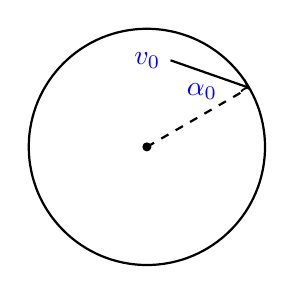
\begin{tikzpicture}
        \draw[thick] (0, 0) circle (1.5cm);
        \draw[fill = black] (0, 0) circle (0.05cm);
        \draw[thick, dashed] (0, 0) -- ++(30:1.5cm);
        \draw[thick, ->] (0.3, 1.1) node[blue, left] {$v_0$} -- (1.3, 0.75);
        \draw (0.7, 0.7) node[blue] {$\alpha_0$};
    \end{tikzpicture}
}  
% Москва, город-2006, 10 класс